\documentclass[conference]{IEEEtran}

\usepackage[T1]{fontenc}
\usepackage[utf8]{inputenc}
\usepackage{cite}
\usepackage{amsmath,amssymb,amsfonts}
\usepackage{graphicx}
\usepackage{booktabs}
\usepackage{array}
\usepackage{multirow}
\usepackage{url}
\usepackage{microtype}
\usepackage[hidelinks]{hyperref}
\usepackage{placeins}
\usepackage{xcolor}
\newcommand{\changed}[1]{\textcolor{blue}{#1}}

\setlength{\textfloatsep}{8pt plus 1pt minus 2pt}
\setlength{\dbltextfloatsep}{8pt plus 1pt minus 2pt}
\setlength{\floatsep}{8pt plus 1pt minus 2pt}
\setlength{\intextsep}{8pt plus 1pt minus 2pt}

\newcolumntype{L}[1]{>{\raggedright\arraybackslash}p{#1}}
\setlength{\emergencystretch}{2em}

\begin{document}

\title{Fault of Our Stars: Behavioral Drivers of
Rating–Sentiment Incongruence}


\maketitle

\begin{abstract}
When people share experiences online, they often express their opinions in two ways: a star rating and a written review. In sentiment analysis, \changed{ratings are widely used as convenient weak labels for textual sentiment}, yet whether the two actually agree is rarely questioned. This study investigates sentiment–rating incongruence, where the sentiment expressed in review text differs from the sentiment implied by the assigned star rating, in the context of Sri Lankan tourism attraction reviews. Rather than treating such mismatches as simple labeling errors, we examine them as evidence of \changed{weak-label unreliability in review-based NLP}. A large dataset of 16,156 attraction reviews from 2010 to 2023 is analyzed using a \changed{transformer-based sentiment pipeline that derives textual sentiment independently of assigned ratings}. Results show that incongruence occurs in 18.6\% of reviews and falls into six directional patterns, with Conservative Rater and Obligatory 5-Star behaviors accounting for the majority of mismatches. Incongruence also varies across venue types, with museums showing the highest prevalence. \changed{Statistical tests, logistic regression, Random Forest, and SHAP are then used as secondary explanatory tools} to identify factors associated with these mismatches. The findings show that venue type, reviewer expertise, review length, and temporal factors contribute to rating–text divergence. Overall, this study demonstrates that \changed{star ratings are not interchangeable with textual sentiment and should be validated before being treated as ground-truth labels in NLP}.
\end{abstract}

\begin{IEEEkeywords}
Sentiment Analysis, \changed{Natural Language Processing}, \changed{Transformer Models}, \changed{Weak Label Reliability}, Rating–Text Incongruence, \changed{Review Mining}, Tourism Reviews.
\end{IEEEkeywords}

\section{Introduction}
Online tourism reviews are an important source of user-generated content for understanding visitor experiences. Most review platforms allow users to express their experience through both a star rating and a written review. In sentiment analysis and review mining, star ratings are often treated as convenient weak labels for textual sentiment \cite{Pang,alaei}. However, this assumption is not always reliable. A high rating does not necessarily mean that the review text is fully positive, and a moderate rating may still contain strongly positive language. \changed{This creates an NLP problem: ratings may introduce noisy or context-biased labels when used as ground truth for sentiment analysis.}

The growth of platforms such as TripAdvisor has expanded tourism review data \cite{George}. Many studies use these reviews to analyze destination image, tourist satisfaction, and consumer behavior. However, the relationship between rating-derived and text-derived sentiment remains insufficiently examined. In many sentiment analysis pipelines, star ratings are used as proxy labels without validating whether the written review expresses the same polarity. \changed{From an NLP perspective, this becomes a weak-supervision problem, where models trained or evaluated using ratings may learn distorted patterns rather than the actual sentiment expressed in language.}

This study examines sentiment--rating incongruence, defined as a mismatch between the sentiment expressed in review text and the sentiment implied by the assigned star rating. These mismatches represent meaningful patterns in how reviewers express their experiences, indicating that rating and text capture different dimensions of the user experience.

Previous studies suggest that rating--text inconsistency is a recurring issue in online reviews \cite{Bigne,Kwon}. However, much of the tourism sentiment analysis literature still relies on ratings as sentiment labels, particularly in hotel and restaurant contexts \cite{alaei,Ameur}. Although aspect-based sentiment analysis and topic modeling have improved the extraction of fine-grained information from review text \cite{Chu2022,Ali}, the broader question of whether ratings reliably represent textual sentiment has received less attention. This gap is especially important in underrepresented tourism contexts, where review behavior may be shaped by local cultural expectations, attraction types, and reviewer experience.

Prior studies in the Sri Lankan context have identified rating-text incompatibility in hotel reviews but mainly approach the problem as one of correcting mismatch using lexicon-based techniques, rather than analyzing it as a \changed{structured NLP weak-label reliability issue}.

Recent transformer-based language models provide an opportunity to study sentiment--rating incongruence more effectively. Models such as BERT, ERNIE, and RoBERTa capture contextual meaning more effectively than traditional lexicon-based approaches \cite{Wen,Puh,Devlin,Sun}. In this study, \changed{transformer-based sentiment inference is used to derive textual sentiment independently from assigned ratings}, allowing review text to be analyzed as a separate linguistic signal.

Using 16,156 Sri Lankan tourism attraction reviews collected between 2010 and 2023 \cite{Sewwandi}, this study investigates how often rating-derived sentiment and NLP-derived textual sentiment diverge, what directional forms these mismatches take, and which contextual and reviewer-level factors are associated with them. Star ratings are grouped into negative, neutral, and positive classes, while textual sentiment is inferred using a transformer-based sentiment pipeline selected through comparative model evaluation. The resulting mismatches are organized into six directional incongruence patterns, moving beyond a simple matched/mismatched classification.

After deriving textual sentiment through transformer-based NLP inference, statistical and machine learning models are used as secondary explanatory tools to examine factors associated with rating--text divergence. \changed{This study makes four contributions: it evaluates star ratings as weak labels for textual sentiment, applies transformer-based sentiment inference independently from ratings, introduces six directional sentiment--rating incongruence patterns, and identifies contextual and reviewer-level drivers of NLP-derived mismatches.}

Overall, this paper argues that sentiment--rating incongruence is not random noise but a systematic and context-dependent signal. For NLP research, the findings highlight the risk of treating star ratings as ground-truth sentiment labels without validation. For tourism review analytics, they show that ratings and written reviews capture different aspects of visitor experience, supporting the need for context-aware sentiment analysis approaches.

\section{Related Work}
The foundational survey by Pang and Lee \cite{Pang} established sentiment analysis as a
major research area and reinforced the assumption that star ratings
broadly reflect textual sentiment. Despite recognized
limitations, this convention remains widely used in tourism research as a
practical weak-labeling strategy. Alaei et al. \cite{alaei} note that ratings are
often treated as weak labels without explicit validation and that the
literature concentrates on hotels and restaurants. Ameur et al. \cite{Ameur} further report limited venue
diversity and restricted geographic coverage, especially
for emerging tourism destinations.

Methodological advances have improved tourism sentiment analysis.
Wen et al. \cite{Wen} demonstrate the effectiveness of transformer-based
models such as BERT \cite{Devlin} and ERNIE \cite{Sun}, while Puh and Bagic Babac \cite{Puh} show
that jointly analyzing sentiment and ratings provides more detailed insight.
Aspect-based and multilingual methods further improve
interpretability by linking sentiment to specific experience components
\cite{Chu2022,Ali}. Zero-shot approaches have also expanded the
feasibility of analyzing under-studied datasets with limited labeled data
\cite{Nawawi}.

This inconsistency appears in regional literature as well. Abeysinghe and Walgampaya \cite{walgampaya} document rating–text incompatibility in hotel reviews in Anuradhapura, while Abeysinghe and Bandara \cite{abeysinghe} extend this finding across five Sri Lankan cities. Both depend on lexicon-based methods and frame mismatch mainly as a correction problem. \changed{In contrast, this study uses transformer-based sentiment analysis and interprets incongruence as a context-dependent NLP weak-label reliability issue.}

Empirical findings on the relationship between ratings and review text remain
mixed. Bigne et al. \cite{Bigne} report general alignment between the two, but also
identify variation across contexts. George and Ramos \cite{George} show that ratings may
exceed text-based sentiment in destination-related reviews, while Kwon et al.
\cite{Kwon} demonstrate that rating--text inconsistency varies by context and
influences perceived review usefulness. These findings suggest that ratings and
text do not always capture the same dimension of experience.

Reviewer characteristics also matter. Chua and Banerjee \cite{Chua} show that
reviewer expertise influences the relationship between ratings and textual
content, while related work links review depth to
perceived usefulness \cite{Chua,Ameur}. These studies indicate that
ratings and text may encode different aspects of user experience and that
inconsistency may be partly shaped by reviewer-level behavior.

Overall, sentiment–rating incongruence remains insufficiently understood in tourism attraction contexts. While recent methods enable large-scale analysis, there is limited evidence on the structure of directional mismatch patterns and their drivers in multi-venue datasets. \changed{This study addresses this gap by analyzing rating–text mismatch as a weak-label reliability problem in NLP.}

\section{Methodology}


\begin{table}[htbp]
\caption{Methodology Overview}
\label{tab:methodology_overview}
\centering
\resizebox{\columnwidth}{!}{%
\begin{tabular}{L{0.4cm}L{2.2cm}L{2.8cm}L{3.2cm}}
\toprule
\textbf{Ph.} & \textbf{Stage} & \textbf{Method / Tool} & \textbf{Output} \\
\midrule
1 & Dataset and Preprocessing       & Rule-based normalization, Feature engineering          & Clean review dataset \\
2 & Sentiment Model Selection    & Comparative evaluation of RoBERTa variants on 1,000 manually labeled reviews; \changed{textual sentiment inferred independently from ratings} & Best performing model selected for full dataset sentiment prediction \\
3 & Variable Construction   & Derived from model output and reviewer data            & Incongruence flag, Pattern type, Reviewer tier \\
4 & Statistical Testing and Predictive Modeling            & Chi-square, Mann--Whitney U, Logit, Random Forest, SHAP & \changed{Secondary explanatory factors and effect sizes} \\
\bottomrule
\end{tabular}%
}
\end{table}

\subsection{Dataset and Preprocessing}

The study used the ``Tourism and Travel Reviews: Sri Lankan Destinations'' dataset from Mendeley Data~\cite{Sewwandi}, which contains 16,156 reviews from 2010 to 2023 across 11 attraction types in Sri Lanka. Missing values and duplicates were checked during preprocessing. Date fields were used to create travel year and review delay, with negative delay values set to zero. Raw location text was processed using rule-based parsing and manual mapping to identify province and district. \textit{Review\_Length} was calculated as the character count of the review text. Star ratings were grouped into three classes:
\begin{itemize}
    \item Negative (1--2$\star$)
    \item Neutral (3$\star$)
    \item Positive (4--5$\star$)
\end{itemize}
This grouping follows common practice in sentiment analysis~\cite{Pang,alaei} and makes the rating scale directly comparable with the three-class sentiment output. Table~\ref{tab:dataset_attributes} presents the source columns used to build the analytical dataset and only the relevant columns used in analysis are presented. \changed{This preprocessing ensured that the sentiment labels, rating classes, temporal variables, and reviewer-level features were constructed consistently before modeling rating--text divergence.}

\begin{table}[htbp]
\caption{Source Columns Used in Analysis}
\label{tab:dataset_attributes}
\centering
\resizebox{\columnwidth}{!}{%
\begin{tabular}{L{3.0cm}L{4.8cm}}
\toprule
\textbf{Feature} & \textbf{Description} \\
\midrule
Location            & Raw location text used to derive province and district \\
Location\_Type      & Type of attraction (museum, beach, temple, etc.) \\
User\_Contributions & Total number of reviews posted by the reviewer \\
Travel\_Date        & Date of the visit; used to derive travel year \\
Published\_Date     & Date of review posting; used to derive review delay \\
Rating              & Star rating used to create Rating\_Class \\
Title               & Review title; combined with text for sentiment inference \\
Text                & Review body; used for sentiment and review length \\
\bottomrule
\end{tabular}%
}
\end{table}

\subsection{Sentiment Model Selection}

\changed{To derive textual sentiment independently from ratings}, four transformer-based sentiment models were evaluated on a manually labeled subset of 1,000 reviews using concatenated review title and body text as input. The data were split into 700 training and 300 testing instances, and the models were compared using accuracy, Macro F1, and weighted F1. \changed{Macro F1 was included because sentiment classes may be imbalanced.} As shown in Table III, the pretrained cardiffnlp/twitter-roberta-base-sentiment model achieved the best overall balance, with the highest accuracy of 0.830 and weighted F1 of 0.805, while maintaining a strong Macro F1 of 0.692. Although the fine-tuned RoBERTa-base model produced a slightly higher Macro F1, its lower accuracy and weighted F1 indicated weaker overall generalization. \changed{Therefore, Cardiff RoBERTa was selected for full-dataset sentiment inference, allowing textual sentiment to be measured independently from star ratings and supporting the NLP objective of testing rating reliability as weak sentiment labels.} \changed{This design also reduces circularity in the analysis because textual sentiment is inferred from review language rather than directly inherited from the rating score.} As a result, \changed{mismatch detection is based on two independently derived signals: rating-derived sentiment and NLP-derived textual sentiment}.
\begin{table}[htbp]
\caption{Sentiment Model Performance (Test Set, $n = 300$)}
\label{tab:sentiment_performance}
\centering
\resizebox{\columnwidth}{!}{%
\begin{tabular}{L{4.2cm}cccc}
\toprule
\textbf{Model} & \textbf{Acc.} & \textbf{Mac. F1} & \textbf{Wt. F1} & \textbf{Decision} \\
\midrule
gosorio/robertaSentimentFT  & 0.730 & 0.281 & 0.616 & Rejected \\
cardiffnlp/twitter-roberta (pretrained) & 0.830 & 0.692 & 0.805 & \textbf{Selected} \\
Fine-tuned Cardiff RoBERTa  & 0.733 & 0.677 & 0.758 & Lower overall fit \\
Fine-tuned RoBERTa-base     & 0.777 & 0.698 & 0.780 & Higher Mac.\ F1 only \\
\bottomrule
\end{tabular}%
}
\end{table}

\subsection{Variable Construction}

After sentiment labeling, raw title and text were removed from further
analysis. \textit{Incongruent} was defined as a mismatch between
\textit{Sentiment} and \textit{Rating\_Class}, while \textit{Pattern} recorded
the six mismatch types. \textit{Reviewer\_Tier} grouped reviewers as follows: Novice (0--5), Casual (6--20), Active (21--100), Expert (101+).

Reviewer tiers were defined by analyzing contribution distribution. The data show strong positive skew (median = 54, max = 9010), with many low-contribution users and a smaller group of highly active reviewers. Thresholds were set at 0–5, 6–20, 21–100, and 101+ to capture distinct engagement levels. This grouping is supported by rating behavior: the Conservative Rater pattern increases from 27.4\% among novice reviewers to 40.4\% among experts, indicating experience-dependent rating practices. These tiers therefore capture both contribution intensity and observable differences in rating–text alignment.


The constructed analytical variables used in this study comprise both target-defining and explanatory features. \textit{Sentiment} is represented as a three-class label derived from model output, while \textit{Rating\_Class} is a three-class label obtained by grouping star ratings (1--5); together, these variables define sentiment–rating incongruence, from which the binary variable \textit{Incongruent} (0/1) is derived as the target outcome. \textit{Pattern} is a six-category variable formed from the interaction between \textit{Sentiment} and \textit{Rating\_Class}, capturing distinct mismatch typologies, and \textit{Reviewer\_Tier} is a four-level ordinal variable based on grouped contribution levels, used as a predictor. Continuous predictors include \textit{log\_review\_length}, computed as the logarithm of review length in characters using $\log(1+x)$, and \textit{log\_review\_delay}, defined as the logarithm of the time gap between visit and posting using $\log(1+x)$. Temporal effects are modeled using \textit{Travel\_Year\_c}, a centered travel year variable, and its squared term \textit{Travel\_Year\_c\textsuperscript{2}}, which captures potential nonlinear time trends. Together, these variables provide a structured representation of textual, behavioral, and temporal factors relevant to the analysis.



\subsection{Statistical Testing and Predictive Modeling}

\changed{After deriving textual sentiment through transformer-based NLP inference}, statistical and machine learning models were used as \changed{secondary explanatory tools} to examine factors associated with rating--text mismatch. \textit{Incongruent} was used as the binary outcome variable, while variables used to define it were excluded from the predictors to avoid data leakage. The final predictor set included venue type, province, reviewer tier, review length, review delay, and travel year terms, with low multicollinearity (max VIF~$= 3.663$).

Chi-square and Mann--Whitney U tests were used for bivariate analysis, with Benjamini--Hochberg correction applied for multiple testing. Logistic regression and logit models were used to examine linear effects and adjusted odds ratios, while Random Forest was used to assess nonlinear relationships. \changed{SHAP was used only as a post hoc interpretation layer} for the Random Forest model, \changed{supporting the explanation of NLP-derived incongruence rather than replacing the main sentiment analysis framework}. Model performance was evaluated using AUC-ROC.

\begin{table}[htbp]
\caption{Modeling and Interpretation Framework}
\label{tab:model_framework}
\centering
\resizebox{\columnwidth}{!}{%
\begin{tabular}{L{1.6cm}L{2.5cm}L{1.4cm}L{2.8cm}}
\toprule
\textbf{Model} & \textbf{Purpose} & \textbf{Metric} & \textbf{Key Detail} \\
\midrule
1A: Logistic Reg.        & Linear baseline performance     & AUC-ROC       & Stratified 80/20 split; balanced classes; 5-fold CV \\
1B: Logit (statsmodels)  & Identifies independent drivers  & 95\% CI       & Unweighted inference model fit on full design matrix \\
2: Random Forest         & Captures complex relationships  & AUC-ROC       & GridSearchCV on training set; same held-out test set \\
SHAP (post hoc)          & Explains model predictions      & Mean $|\phi|$ & TreeExplainer on the best Random Forest \\
\bottomrule
\end{tabular}%
}
\end{table}

 

\section{Results}
\subsection{Prevalence and Six-Pattern Typology}

Each incongruence type reflects a directional mismatch between rating and sentiment polarity. Pattern names were derived from their defining characteristics: \textit{Conservative Rater} pairs positive sentiment with neutral ratings; \textit{Obligatory 5-Star} pairs neutral sentiment with positive ratings; \textit{Frustrated Neutral} pairs negative sentiment with neutral ratings; \textit{Polite Inflator} pairs negative sentiment with positive ratings; \textit{Harsh Deflator} pairs neutral sentiment with negative ratings; and \textit{Punitive Rater} pairs positive sentiment with negative ratings.

Among the reviews analyzed, 3,005 were identified as incongruent, giving an overall prevalence of 18.6\%, or roughly one in five reviews. Fig. 1 shows that incongruence follows a six-pattern typology. The two most common patterns, \textit{Conservative Rater} (38.4\%) and \textit{Obligatory 5-Star} (28.3\%), together account for 66.7\% of all incongruent reviews. In addition, \textit{Frustrated Neutral} and \textit{Polite Inflator} account for a further 24.2\% of incongruent cases, showing that negative textual sentiment is often paired with non-negative ratings. \changed{This directional structure indicates that rating-derived labels introduce systematic, rather than random, noise into sentiment analysis tasks.} \changed{The dominance of a few directional patterns also suggests that incongruence follows repeated linguistic-rating behaviors rather than isolated annotation errors.} \changed{This makes the pattern typology useful for interpreting how numerical ratings and written sentiment diverge in review-mining datasets.}

\begin{figure}[htbp]
\centering
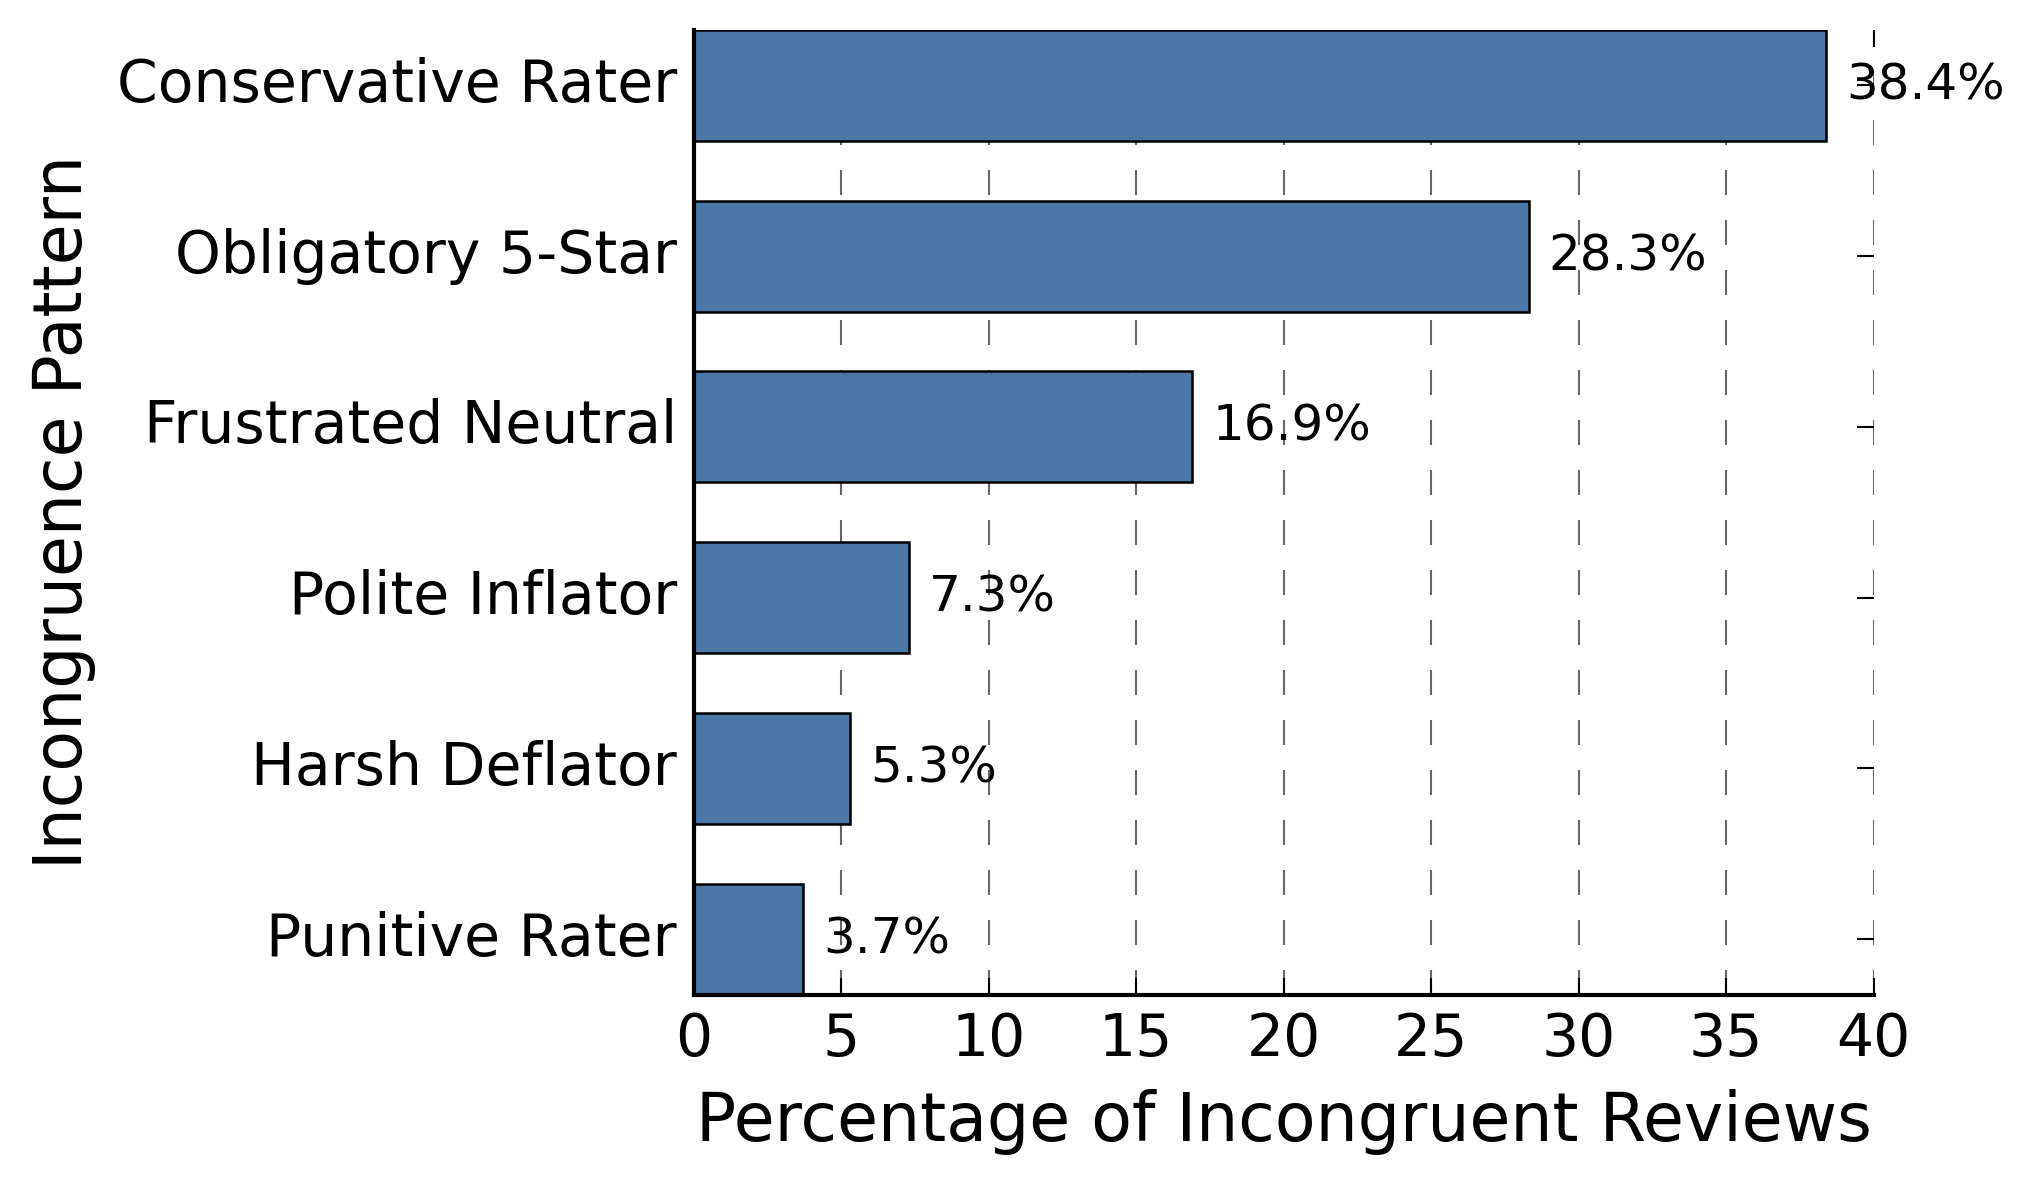
\includegraphics[width=\columnwidth]{fig_incongruence_patterns.png}
\caption{Distribution of the six directional incongruence patterns.}
\label{fig:incongruence_patterns}
\end{figure}

\subsection{Variation Across Venue Types}
Incongruence rates were compared across 11 attraction categories to assess
contextual variation. The Chi-square test showed a statistically significant
association between venue type and incongruence, with a small but meaningful
effect size ($\chi^2(10) = 125.85$, $p < 0.001$; Cramer's V = 0.088). As shown
in Fig.~\ref{fig:venue_incongruence_rate}, National Parks had the lowest
incongruence rate (12.8\%), whereas Museums had the highest (26.3\%). Overall, the variation across
venue types indicates that rating--text mismatch is not evenly distributed, but
differs by review context.

\begin{figure}[htbp]
\centering
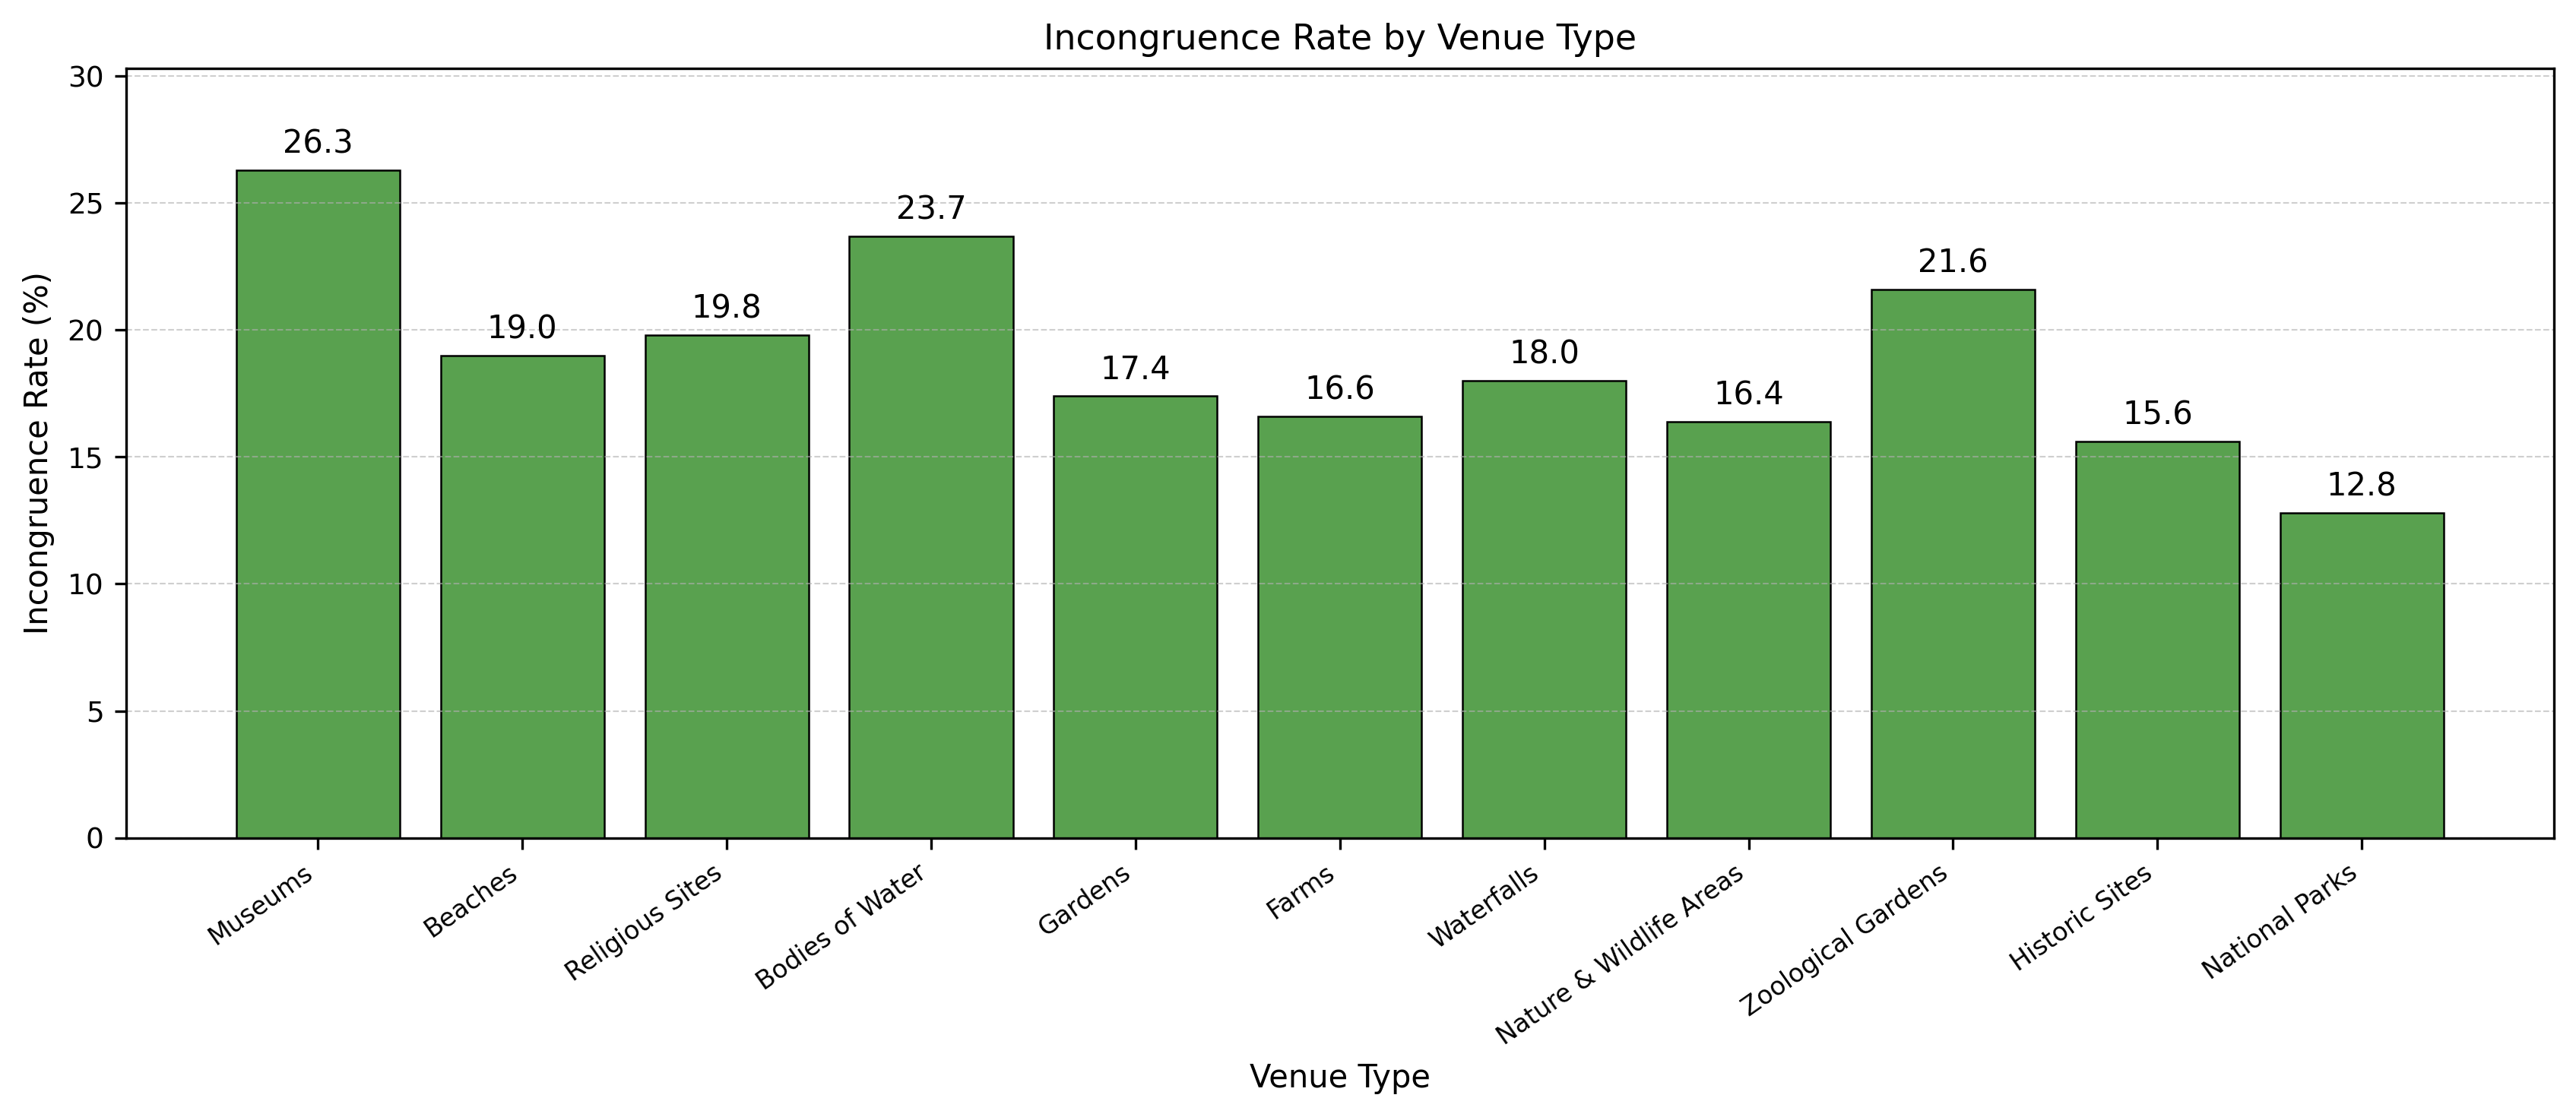
\includegraphics[width=\columnwidth]{fig_venue_incongruence_rate.png}
\caption{Incongruence rate by venue type.}
\label{fig:venue_incongruence_rate}
\end{figure}

\subsection{Predictors of Incongruence}
Bivariate screening with Benjamini--Hochberg correction was used to identify
predictors associated with incongruence. As shown in
Table~\ref{tab:bivariate_screening}, reviewer tier, province, travel year, and
review length remained significant after correction,
while review delay was not significant ($q = 0.7503$). Expert reviewers were
1.97 times more likely than novices to produce incongruent reviews. In
addition, incongruent reviews were longer at the median than congruent reviews
(296 vs. 279 characters). These findings indicate that both reviewer
characteristics and review content are associated with sentiment--rating
mismatch, although multivariable modeling is needed to test their independent
effects.

Fig.~\ref{fig:reviewer_expertise_patterns} further illustrates the reviewer expertise effect for selected mismatch patterns, showing that Conservative Rater becomes more common among expert reviewers, while Harsh Deflator becomes less common.

\begin{table}[htbp]
\caption{Bivariate Predictor Screening with Benjamini--Hochberg FDR Correction}
\label{tab:bivariate_screening}
\centering
\resizebox{\columnwidth}{!}{%
\begin{tabular}{L{2.0cm}L{1.8cm}L{1.3cm}L{1.3cm}L{1.0cm}}
\toprule
Predictor & Test Statistic & Raw $p$ & $q$-value & Retained \\
\midrule
Reviewer Tier & $\chi^2(3)=85.99$ & $1.59\times10^{-18}$ & $7.94\times10^{-18}$ & Yes \\
Province & $\chi^2(7)=49.10$ & $2.17\times10^{-8}$ & $3.62\times10^{-8}$ & Yes \\
Travel Year & Mann--Whitney & $7.73\times10^{-11}$ & $1.93\times10^{-10}$ & Yes \\
Review Length & Mann--Whitney & 0.0011 & 0.0014 & Yes \\
Review Delay & Mann--Whitney & 0.7503 & 0.7503 & No \\
\bottomrule
\end{tabular}%
}
\end{table}

\subsection{Model-Based Analysis and Interpretation}
\text{1) Model 1A -- Logistic Regression:}
A class-balanced logistic regression model was used as a linear baseline. It
achieved a mean cross-validated AUC of $0.5890 \pm 0.0093$ and a test AUC of
0.5840, indicating modest but stable predictive performance. This suggests that
incongruence is only partly explained by the observed variables.

\text{2) Model 1B -- Explanatory Logit:}
The explanatory logit model was used to identify independent predictors of
incongruence. Based on 95\% confidence intervals, 19 predictors were
statistically significant. Venue type, reviewer expertise, review length, and
travel year showed important effects, while review delay had only a weak
negative association. Overall, the model shows that incongruence is shaped by
structural, behavioral, and temporal factors.

\text{3) Model 2 -- Random Forest (Nonlinear Structure Test):}
A Random Forest model was applied to capture nonlinear relationships and
interactions. It achieved a test AUC of 0.6095, which was slightly higher than
logistic regression. This indicates that nonlinear effects are present, although
their contribution is modest.

\text{4) SHAP Analysis}
SHAP was used as a post hoc interpretation layer for the Random Forest model to identify influential features behind NLP-derived incongruence. The results were broadly consistent with the logit model, highlighting review length, reviewer expertise, travel year, review delay, and venue type as influential factors. SHAP therefore supports interpretation of nonlinear patterns rather than replacing the main sentiment analysis framework.

Temporal effects indicate a modest but consistent decline in sentiment–rating incongruence over time. The linear travel year term shows a significant negative association (Travel\_Year\_c: OR = 0.946, CI < 1), suggesting that more recent reviews are less likely to be incongruent. In contrast, the quadratic term (Travel\_Year\_c²: OR = 0.995) is not statistically significant, providing no evidence of nonlinear temporal effects and indicating an approximately linear trend. SHAP analysis further supports this finding, identifying Travel\_Year\_c as an influential predictor (mean |SHAP| = 0.0219) and confirming the overall direction of the effect. This suggests that, over time, reviewers are expressing their opinions more consistently, with written sentiment aligning more closely with their ratings.


\section{Discussion}
\subsection{Structured Incongruence}

The incongruence rate of 18.6\% shows that rating--text mismatch is systematic rather than random. Ratings capture overall judgments, while review text captures more specific details of the visitor experience. For sentiment analysis, a numerical score may compress a complex experience into a single label, while the written review can express mixed or context-dependent sentiment.

The six-pattern structure further shows that incongruence is directional rather than accidental. \textit{Conservative Rater} and \textit{Obligatory 5-Star} patterns dominate the mismatched cases, indicating that reviewers do not simply make random rating errors. \changed{For NLP pipelines, this means that star ratings do not function equally across contexts as weak sentiment labels.} \changed{Using them without validation can introduce systematic label noise into sentiment analysis models.} Ratings and textual sentiment therefore capture different dimensions of experience, and treating them as interchangeable signals creates modeling risk. \changed{This supports the use of review text as an independent sentiment signal when building or evaluating review-mining systems.} \changed{It also suggests that rating-based labels should be checked for domain-specific bias before being used for supervised sentiment classification.}

\subsection{\changed{Conservative Rating as Structured Label Noise}}

The Conservative Rater pattern further reinforces structural incongruence. Positive textual sentiment paired with moderate ratings accounts for 38.4\% of incongruent reviews. Reviewers temper their numerical scores relative to their written sentiment rather than align them fully.
Prevalence of this pattern rises from 27.4\% (novice reviewers) to 40.4\% (expert reviewers), showing that rating behavior becomes more calibrated with experience. Experienced reviewers apply stricter standards, reserving high ratings for exceptional experiences while maintaining positive text sentiment. This indicates incongruence reflects deliberate practice, not inconsistency. In short, \changed{rating-supervised sentiment models may learn misleading labels when positive textual sentiment is paired with moderate ratings}, \changed{creating structured label noise when ratings are used as ground-truth sentiment labels}. Accounting for reviewer expertise is therefore critical when interpreting rating-text relationships in NLP.

\subsection{\changed{Location Type as a Structural Moderator of Label Reliability}}
Location type affects rating–text reliability. Museums are over twice as likely to be incongruent compared with national parks (Adjusted OR = 2.386), with similar patterns for beaches, inland waterbodies, zoological gardens, and waterfalls. This suggests that some attraction types are harder to evaluate using a single numerical score. Museums and cultural sites often involve layered experiences, where visitors may describe positive exhibits, heritage value, or emotional significance while also mentioning issues such as crowding, pricing, accessibility, or facilities.

These findings indicate that \changed{star-rating reliability is context-dependent} rather than uniform across all review types. Rating-derived labels may therefore introduce systematic bias when treated as equally reliable sentiment labels across different tourism contexts. For NLP, this supports the need for \changed{context-aware sentiment modeling} that validates whether rating-derived sentiment and textual sentiment are aligned before using ratings as ground-truth labels. \changed{In practical NLP applications, this means that attraction categories may require different levels of label validation before ratings are reused as sentiment labels.}

\subsection{Complementary Roles of Linear and Nonlinear Models}
Results show that linear and nonlinear models offer complementary insights into sentiment–rating incongruence. Logistic regression (AUC = 0.584) provides a stable and interpretable baseline, identifying 19 significant predictors, while Random Forest achieves a modest improvement (AUC = 0.6095), confirming nonlinear effects. However, the limited improvement suggests that nonlinear relationships are present but not dominant. These models support explanation of NLP-derived mismatch rather than strong predictive power, as rating–text divergence is influenced by contextual and reviewer-level factors not fully captured by structured metadata alone.


\subsection{Review Delay and Reviewer Expertise Effects}

Review delay plays a limited role in sentiment–rating incongruence, showing no significance in bivariate analysis and only a weak negative association (OR = 0.960). In contrast, reviewer expertise is more influential, with experts exhibiting more conservative and fewer harsh rating behaviors. This suggests that mismatch is shaped more by reviewer-dependent rating practices than by the time gap between visit and review publication. For sentiment analysis, this creates systematic label noise when ratings are treated as ground truth because experienced reviewers may write positive text while assigning moderate ratings based on stricter personal standards.



\begin{figure}[htbp]
\centering
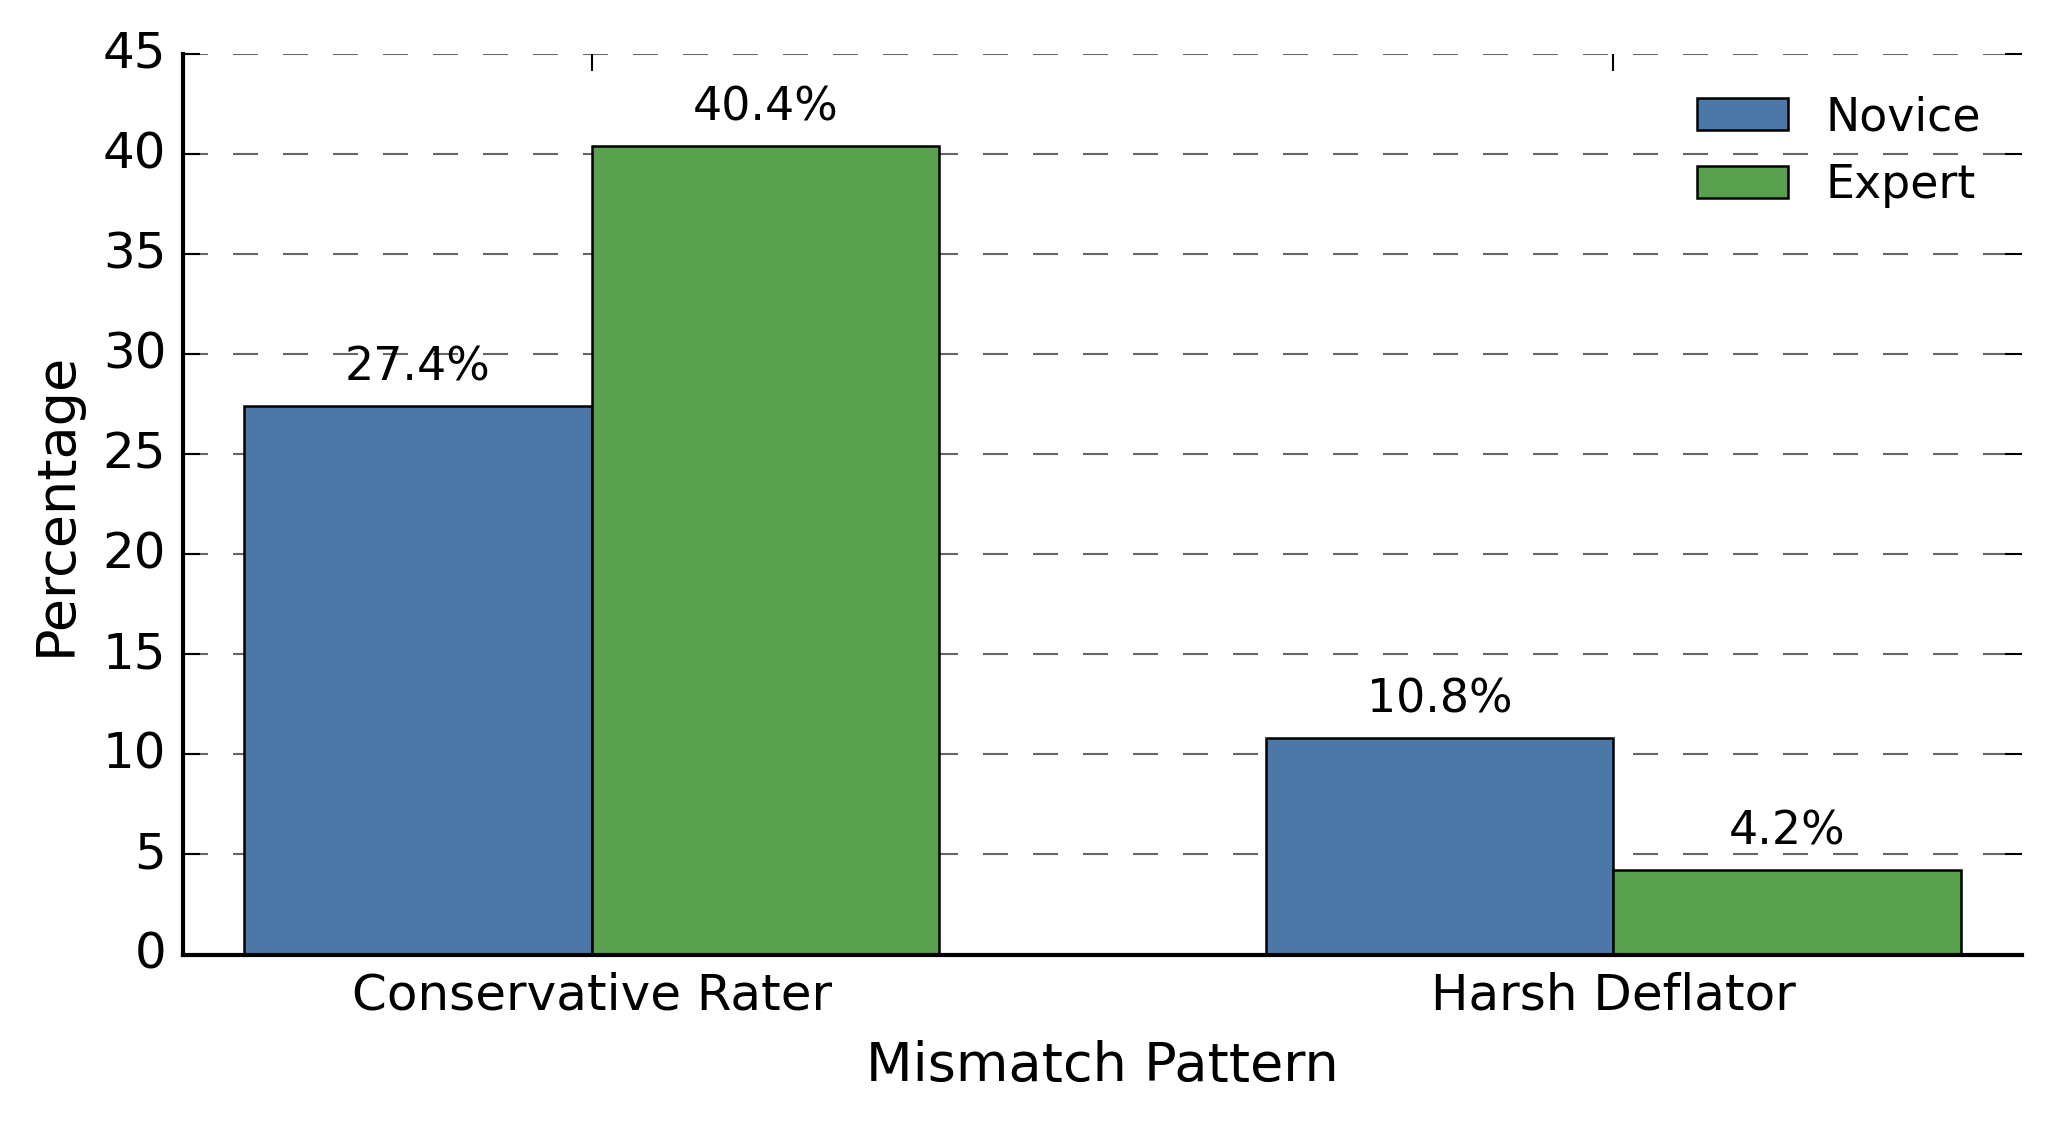
\includegraphics[width=\columnwidth]{fig_reviewer_expertise_patterns.png}
\caption{Selected incongruence patterns by reviewer expertise, showing higher Conservative Rater prevalence and lower Harsh Deflator prevalence among expert reviewers.}
\label{fig:reviewer_expertise_patterns}
\end{figure}

\FloatBarrier


\section{Conclusion}
Sentiment–rating incongruence in tourism reviews is systematic rather than random. Using transformer-based sentiment inference, this study showed that 18.6\% of reviews contain rating–text mismatch forming six directional patterns. The findings show that reviewer expertise, review length, venue type, and temporal factors influence rating–text divergence. More importantly, \changed{star ratings and textual sentiment are not interchangeable signals}. \changed{This distinction is especially important for datasets where ratings are used automatically as training labels.}

For NLP research, the main implication is that \changed{star ratings should not be treated as ground-truth sentiment labels without validation}. \changed{Rating-derived sentiment labels may introduce systematic label noise} when the written review expresses a different sentiment polarity from the assigned score. This study therefore supports the need for \changed{context-aware sentiment analysis methods that evaluate weak-label reliability} before model training or evaluation.

The study also contributes to tourism review analytics by showing that visitor evaluations are expressed differently through ratings and written text. The framework can be applied to other review platforms containing both numerical ratings and textual feedback. \changed{Future work may compare RoBERTa-based sentiment inference with lexicon-based baselines such as VADER or TextBlob and traditional TF-IDF classifiers}, and test whether these patterns generalize across other domains.

 

\bibliographystyle{IEEEtran}
\bibliography{references}

\end{document}